\documentclass{article}
\usepackage{graphicx} % Required for inserting images
\usepackage{siunitx}

\title{ideas}
\author{r.reyes }
\date{December 2023}

\begin{document}

\maketitle

\section{Introducción}

En el medio interestelar hay muchas hay grandes regiones de nubes moleculares frías en las cuales se pueden formar estrellas a partir del colapso gravitacional y estas estrellas interactúan con el medio que la rodea. Cuando hay grandes concentraciones de gas y polvo en el medio se forman los \textit{glóbulos}, inhomogeneidades en el medio, que se cree que se pueden formar por colapso gravitacional, inestabilidades termales o por turbulencia. 

Estos glóbulos interactúan con la radiación UV de estrellas jóvenes masivas, como estrellas tipo O, en regiones de formación estelar masivas o en nebulosas alrededor de estrellas. Durante esta interacción se forma un frente de ionización, el cuál podemos ver en la mayoría de los casos. Dependiendo de que tan intenso sea el flujo radiativo por parte de la o las estrellas, en algunas ocasiones podemos ver un flujo fotoevaporativo por parte del glóbulo que es causado por la radiación incidente.

Los primeros glóbulos fueron observados por Bart Bok en 1940, estos glóbulos son nubes oscuras, relativamente pequeños comparados con otras regiones de formación estelar, que tienen gran cantidad de gas y polvo. Estos glóbulos contienen principalmente hidrógeno molecular en su interior, así como también pueden tener otras moléculas, metales e incluso algunos silicatos. Si bien puede tener formación estelar en su interior no podemos ver la radiación UV de las estrellas masivas ya que es absorbida por el hidrógeno atómico y el polvo, por eso que se ven oscuras. Sin embargo, estos pueden ser radiados externamente, en regiones de formación estelar, por estrellas jóvenes masivas que se están formando cerca, y en algunos casos podemos ver el frente de ionización.

\begin{figure}[h]
    \centering
    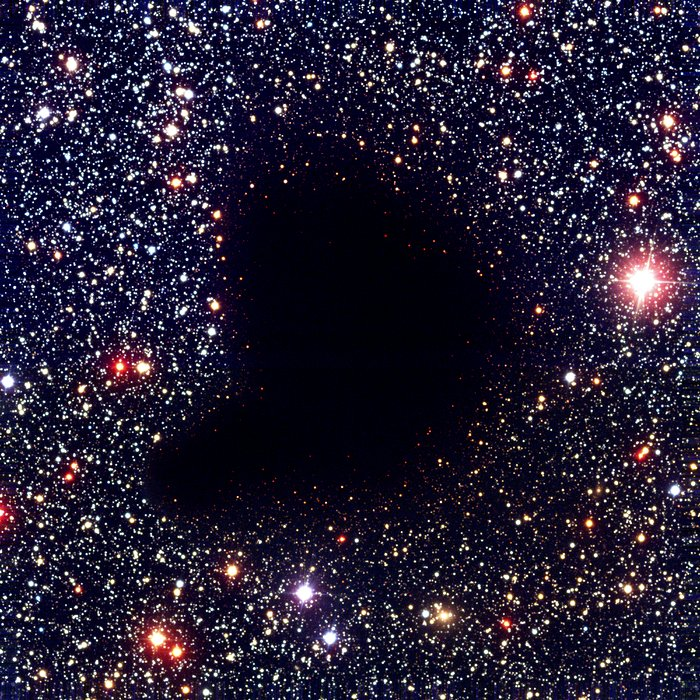
\includegraphics[width=0.75\textwidth]{images Chapter 1/C1_Bok_globule.jpg}
    \caption{Imagen de Banard 68, un ejemplo de un glóbulo de Bok, visto con Very Large Telescope FORS1 en 440 nm, 557 nm y 768 nm. Se puede apreciar una zona oscura y lo que pareciera ser enrojecimiento de las estrellas por polvo en la superficie del glóbulo.}
    \label{fig:zones}
\end{figure}

Esta interacción entre estrellas y glóbulos se puede dar a diferentes escalas, lo que nos da una gran variedad de estructuras. Entre las de mayor tamaño se encuentran lo que parecen ser columnas, pilares o trompas de elefantes, como se les conoce en la literatura, que llegan a tener un tamaño de $\sim$\SI{0.6}{pc} y una densidad del orden de \SI{e3}{cm^{-3}}. En algunas ocasiones tienden a llamar glóbulo en la literatura a los que, al igual que lo anterior a mencionado, tienen una gran estructura también, pero son más densos, $\sim$ \SI{e4}{cm^{-3}}. Esta interacciones también se puede dar dentro de regiones HII, en algunos casos como outflows bipolares.

\begin{figure}[h]
    \centering
    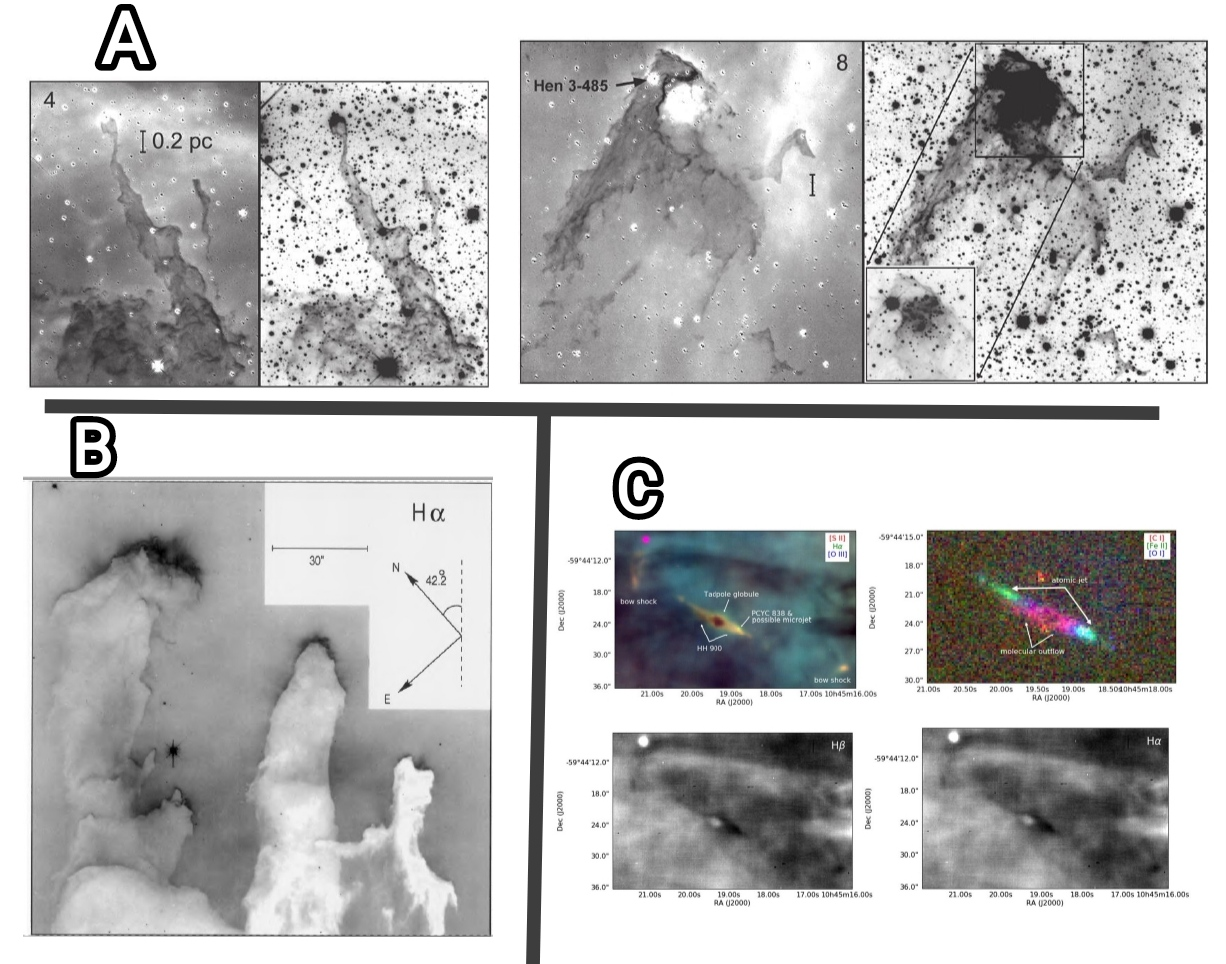
\includegraphics[width=1 \textwidth]{images Chapter 1/C1_Pillars.jpg}
    \caption{En \textbf{A} vemos dos ejemplos de pilares, donde la imagen derecha de cada ejemplo es vista a 2.12$\mu$m (\SI{}{H_2}), y la imagen izquierda es \SI{}{H_2-Br_{\gamma}} (Hartigan et al. 2015). \textbf{B}, ejemplo de una trompa de elefante, es una imagen de M16 tomada con WFPC2 con e filtro F656N, los \SI{30}{\arcsecond} corresponden \SI{9e17}{cm} (\SI{.29}{pc}) (J. Jeff Hester et al. 1996 ). \textbf{C} es el outflow de Tadpole globule, el cual consta del sistema HH900 jet+outflow, la imagen de abajo es vista en \SI{}{H_\alpha} con el continuo 
    (Megan Reiter et al. 2019). }
    \label{fig:zones}
\end{figure}

En escalas más pequeñas están lo que se conoce como EGGs (Evaporating Gaseous Globule) y los proplyds, en escalas de $\sim$\SI{0.1}{pc}. 

No solo se da en regiones de formación estelar, como ya hemos dicho, también hay dentro de nebulosas alrededor de estrellas evolucionadas donde se les conoce más comúnmente como \textit{nudos}, los cuales estudiaremos más a fondo en este trabajo.

\begin{figure}[h]
    \centering
    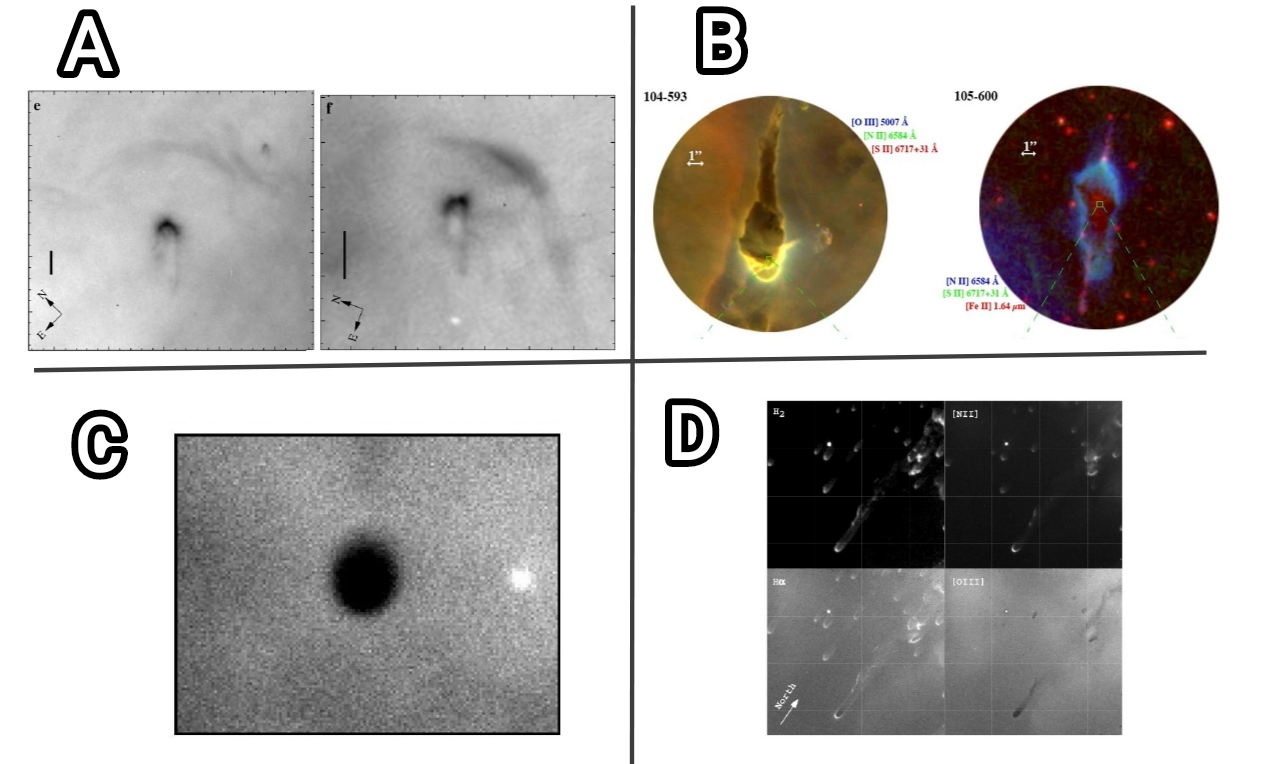
\includegraphics[width=1 \textwidth]{images Chapter 1/C1_Globulettes.jpg}
    \caption{En \textbf{A} vemos proplyds con su bowchock en Orion tomado con HST planetary camera, la barra negra indica una medida de \SI{1}{\arcsecond} que corresponde a 430 AU (García-Arredondo et al. 2001). \textbf{B} son ejemplos de EGGs en Carina, tomado con WFC3, ACS, WFPC2 (Mesa-Delgado et al. 2016). \textbf{C} es el globulette denso RN88 visto en \SI{}{H_\alpha} con un diametro de \SI{6}{\arcsecond} en la nebulosa de Rosette (G.F. Gahm et al. 2013). \textbf{D} son ejemplos de nudos en la nebulosa de la Hélice, los mosaicos tienen una medida de \SI{47.5}{\arcsecond}$\times$\SI{44.8}{\arcsecond} (O'Dell et al. 2007). }
    \label{fig:zones}
\end{figure}


\section{Flujos de fotoevaporación ionizada}


\end{document}
